\documentclass[12pt]{article}
\usepackage[utf8]{inputenc}

\usepackage{lmodern}

\usepackage{enumitem}
\usepackage[margin=2cm]{geometry}

\usepackage{amsmath, amsfonts, amssymb}
\usepackage{graphicx}
%\usepackage{subfigure}
\usepackage{tikz}
\usepackage{pgfplots}
\usepackage{multicol}

\usepackage{comment}
\usepackage{url}
\usepackage{calc}
\usepackage{subcaption}
\usepackage[indent=0pt]{parskip}
\usepackage{animate}

\usepackage{array}
\usepackage{blkarray,booktabs, bigstrut}
\usepackage{bigints}

\pgfplotsset{compat=1.16}

% MATH commands
\newcommand{\ga}{\left\langle}
\newcommand{\da}{\right\rangle}
\newcommand{\oa}{\left\lbrace}
\newcommand{\fa}{\right\rbrace}
\newcommand{\oc}{\left[}
\newcommand{\fc}{\right]}
\newcommand{\op}{\left(}
\newcommand{\fp}{\right)}

\newcommand{\bi}{\mathbf{i}}
\newcommand{\bj}{\mathbf{j}}
\newcommand{\bk}{\mathbf{k}}
\newcommand{\bF}{\mathbf{F}}

\newcommand{\mR}{\mathbb{R}}

\newcommand{\ra}{\rightarrow}
\newcommand{\Ra}{\Rightarrow}

\newcommand{\sech}{\mathrm{sech}\,}
\newcommand{\csch}{\mathrm{csch}\,}
\newcommand{\curl}{\mathrm{curl}\,}
\newcommand{\dive}{\mathrm{div}\,}

\newcommand{\ve}{\varepsilon}
\newcommand{\spc}{\vspace*{0.5cm}}

\DeclareMathOperator{\Ran}{Ran}
\DeclareMathOperator{\Dom}{Dom}

\newcommand{\exo}[1]{\noindent\textcolor{red}{\fbox{\textbf{Problem {#1}}}\hrulefill}\\}
\newcommand{\qu}[4]{\noindent\textcolor{#4}{\fbox{\textbf{Section {#1} | Problem {#2}}} \hrulefill{{\fbox{\textbf{{#3} Points}}}}\\}}

\newcommand{\semester}{Spring 2023}

\newcommand{\CVup}{%

\begin{tikzpicture}
\draw[black, <->, >=latex] (-0.33, 0.5) .. controls (-0.125, 0) and (0.125, 0) .. (0.33, 0.5);
\end{tikzpicture}}

\newcommand{\CVupInc}{%
\begin{tikzpicture}
\draw[black, ->, >=latex] (0,0) .. controls (0.2, 0) and (0.4, 0.2) .. (0.5, 0.5);
\end{tikzpicture}}

\newcommand{\CVupDec}{%
\begin{tikzpicture}[rotate=270]
\draw[black, ->, >=latex] (0,0) .. controls (0.2, 0) and (0.4, 0.2) .. (0.5, 0.5);
\end{tikzpicture}}

\newcommand{\CVdown}{%
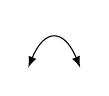
\begin{tikzpicture}
\draw[black, <->, >=latex] (-0.33, -0.5) .. controls (-0.125, 0) and (0.125, 0) .. (0.33, -0.5);
\end{tikzpicture}}

\newcommand{\CVdownInc}{%
\begin{tikzpicture}
\draw[black, ->, >=latex] (-0.5, -0.5) .. controls (-0.5, -0.3) and (-0.5, -0.1) .. (0,0);
\end{tikzpicture}}

\newcommand{\CVdownDec}{%
\begin{tikzpicture}[rotate=-90]
\draw[black, ->, >=latex] (-0.5, -0.5) .. controls (-0.5, -0.3) and (-0.5, -0.1) .. (0,0);
\end{tikzpicture}}

\begin{document}
	\noindent \hrulefill \\
	MATH-241 \hfill Pierre-Olivier Paris{\'e}\\
	Solutions Section 4-3 \hfill \semester \\\vspace*{-1cm}
	
	\noindent\hrulefill
	
	\spc	
	
	\exo{2, (a) and (c)}
	\begin{enumerate}
	\item[(a)] We have $g(0) = 0$, $g(1) = 1/2$, $g(2) = 0$, $g(3) = -1/2$, $g(4) = 0$, $g(5) = 1/2$, and $g(6) = 1$.
	\item[(c)] By the FTC part I, we have $g'(x) = f(x)$. We see that $g'(x)$ doesn't exist when $x = 2$ and $x = 6$, and is zero at $x = 1$ and $x = 3$. Those are the critical points. We can use the closed interval method to find the maximum and minimum value.
		\begin{itemize}
		\item The maximum value is the $\max \{ g(0) , g(1) , g(2) , g(3) , g(6) \} = 1$.
		\item The minimum value is the $\min \{ g(0) , g(1) , g(2) , g(3) , g(6) \} = -1/2$.
		\end{itemize}
	\end{enumerate}
	
	\spc
	
	\exo{8}
	\\
	By the Fundamental Theorem of Calculus, we immediately have
		\begin{align*}
		g'(x) = \cos (x^2) .
		\end{align*}
		
	\spc
	
	\exo{10}
	\\
	Again, from the Fundamental Theorem of Calculus, we have
		\begin{align*}
		h'(u) = \frac{\sqrt{t}}{t + 1} .
		\end{align*}
		
	\spc
	
	\exo{12}
	\\
	Using a property of the integral, we can rewrite $R(y)$ as
		\begin{align*}
		R(y) = - \int_2^y t^3 \sin (t) \, dt .
		\end{align*}
	Therefore, using the FTC, we obtain
		\begin{align*}
		R'(y) = - y^3 \sin (y) .
		\end{align*}
		
	\spc
	
	\exo{14}
	\\
	Write $H(x)$ for $\displaystyle \int_1^x \frac{z^2}{z^4 + 1} \, dz$. Then the function $h(x)$ can be rewritten as
		\begin{align*}
		h(x) = H (\sqrt{x}) .
		\end{align*}
	From the Chain Rule, we find that $h' (x) = H'(\sqrt{x}) \frac{d}{dx} (\sqrt{x})$. Using the FTC, we know that 
		\begin{align*}
		H'(x) = \frac{x^2}{x^4 + 1}
		\end{align*}
	and therefore, we obtain
		\begin{align*}
		h'(x) = \frac{(\sqrt{x})^2}{(\sqrt{x})^4 + 1} \Big( \frac{d}{dx} (\sqrt{x}) \Big) = \frac{1}{2 \sqrt{x}} \frac{x}{x^2 + 1}  = \frac{\sqrt{x}}{2 (x^2 + 1)} .
		\end{align*}
		
	\spc
	
	\exo{18}
	\\
	We rewrite the expression of $y$ as
		\begin{align*}
		y = - \int_{1}^{\sin x} \sqrt{1 + t^2} \, dt .
		\end{align*}
	Writing $Y(x) = \displaystyle \int_1^x \sqrt{1 + t^2} \, dt$, we can rewrite $y$ as
		\begin{align*}
		y(x) = Y(\sin (x)) .
		\end{align*}
	From the Chain Rule, we obtain
		\begin{align*}
		y' (x) = Y'(\sin (x)) \frac{d}{dx} \big( \sin (x) \big) .
		\end{align*}
	Using the FTC, we see that
		\begin{align*}
		Y'(x) = \sqrt{1 + x^2}
		\end{align*}
	and replacing $x$ by $\sin (x)$, we obtain
		\begin{align*}
		y' (x) = \big( \sqrt{1 + \sin^2 (t)} \big) \cos (x)
		\end{align*}
		
	\spc
	
	\exo{20}
	\\
	An antiderivative of $x^{100}$ is $x^{101}/101$. Thus, by FTC part 2, we have
		\begin{align*}
		\int_{-1}^1 x^{100} \, dx = \left. \frac{x^{101}}{101} \right|_{-1}^1 = \frac{2}{101} .
		\end{align*}
	
	\spc
	
	\exo{22}
	\\
	Using linearity, we have
		\begin{align*}
		\int_0^1 (1 - 8v^3 + 16v^7 ) \, dv = \int_0^1 \, dv - 8 \int_0^1 v^3 \, dv + 16 \int_0^1 v^7 \, dv .
		\end{align*}
	Using the part 2 of the FTC, we have
		\begin{align*}
		\int_0^1 (1 - 8v^3 + 16v^7 ) \, dv = \left. v \right|_0^1 - 8 \left. \frac{v^4}{4} \right|_0^1 + 16 \left. \frac{v^8}{8} \right|_0^1 = 1 - 2 + 2 = 1 .
		\end{align*}
		
	\spc
	
	\exo{28}
	\\
	We simply the integrand:
		\begin{align*}
		(4 - t) \sqrt{t} = 4 \sqrt{t} - t^{3/2} .
		\end{align*}
	An antiderivative of this last function is
		\begin{align*}
		\frac{8}{3} t^{3/2} - \frac{2}{5} t^{5/2} .
		\end{align*}
	Therefore, from the FTC, we have
		\begin{align*}
		\int_0^4 (4 - t)\sqrt{t} \, dt &= \left. \big( \tfrac{8}{3} t^{3/2} - \tfrac{2}{5} t^{5/2} \big) \right|_{0}^4  \\
		&= \big( \tfrac{8}{3} (4)^{3/2} - \tfrac{2}{5} (4)^{5/2} \big) - \big( \tfrac{8}{3} (0)^{3/2} - \tfrac{5}{2} (0)^{5/2} \big) \\
		&= \frac{64}{3} - \frac{64}{5} \\
		&= \frac{64}{15} (5 - 3) \\
		&= \frac{128}{15} .
		\end{align*}
	
	\spc
	
	\exo{30}
	\\
	We rewrite the expression of the integrand as
		\begin{align*}
		(3u - 2) (u + 1) = 3u^2 + u - 2 .
		\end{align*}
	An antiderivative for this integrand is
		\begin{align*}
		u^3 + \frac{u^2}{2} - 2u .
		\end{align*}
	Therefore, from the FTC, we get
		\begin{align*}
		\int_{-1}^2 (3u - 2) (u + 1) \, du &= \left. \big( u^3 + \tfrac{1}{2} u^2 - 2u \big) \right|_{-1}^2 \\
		&= \big( 8 + 2 - 4 \big) - \big( -1 + \tfrac{1}{2} + 2 \big) \\
		&= 6 - \tfrac{3}{2} \\
		&= \tfrac{9}{2} .
		\end{align*}
	
	\spc
	
	\exo{34}
	\\
	We have $(s^4 + 1)/s^2 = s^2 + 1/s^2$. Thus,
		\begin{align*}
		\int_1^2 \frac{s^4 + 1}{s^2} \, ds = \int_1^2 s^2 \, ds + \int_1^2 (1/s^2) \, ds = \left. \frac{s^3}{3} \right|_1^2 + \left. \frac{-1}{s} \right|_1^2 = \frac{8 - 1}{3} + 1/2 = 11/6 .
		\end{align*}
		
	\spc
		
	\exo{35}
	\\
	The expression of the integrand can be rewritten as
		\begin{align*}
		\frac{v^5 + 3v^6}{v^4} = v + 3v^2 .
		\end{align*}
	An antiderivative for this integrand is
		\begin{align*}
		\frac{v^2}{2} + v^3 .
		\end{align*}
	Therefore, form the FTC, we have
		\begin{align*}
		\int_1^2 \frac{v^5 + 3v^6}{v^4} \, dv &= \left. \big( \tfrac{1}{2} v^2 + v^3 \big) \right|_{1}^2 \\
		&= \big( 2 + 8 \big) - \big( \tfrac{1}{2} + 1 \big) \\
		&= 10 - \tfrac{3}{2} \\
		&= \tfrac{17}{2} .
		\end{align*}
		
	\spc
	
	\exo{38}
	\\
	We divide the integral in two pars:
		\begin{align*}
		\int_{-2}^2 f(x) \, dx = \int_{-2}^0 f(x) \, dx  + \int_0^2 f(x) \, dx .
		\end{align*}
	According to the definition of the function $f(x)$, we have
		\begin{align*}
		\int_{-2}^2 f(x) \, dx = \int_{-2}^0 2 \, dx + \int_0^2 (4 - x^2) \, dx = 4 + 8 - 8/3 .
		\end{align*}
	So the final answer is $28/3$.
	
	\spc
		
	\exo{54}
	\\
	We rewrite $g(x)$ as followed:
		\begin{align*}
		g(x) = \int_{1 - 2x}^0 t \sin t \, dt + \int_0^{1 + 2x} t \sin t \, dt = -\int_0^{1- 2x} t \sin t \, dt + \int_0^{1 + 2x} t \sin t \, dt .
		\end{align*}		
	Write
		\begin{align*}
		G(x) = \int_0^x t \sin t \, dt
		\end{align*}
	so that
		\begin{align*}
		g(x) = -G(1 - 2x) + G(1 + 2x) .
		\end{align*}				
	Using the Chain Rule, we get
		\begin{align*}
		g'(x) = -G'(1 - 2x) \frac{d}{dx} (1 - 2x) + G'(1 + 2x) \frac{d}{dx} (1 + 2x) .
		\end{align*}
	From the FTC, we have
		\begin{align*}
		G'(x) = x \sin x
		\end{align*}
	so that
		\begin{align*}
		g'(x) = 2(1 - 2x) \sin (1 - 2x) + 2 (1 + 2x) \sin (1 + 2x) .
		\end{align*}
	We can simply this expression using some trig. identities. In $g(x)$, we have the expression
		\begin{align*}
		2 \sin (1 - 2x) + 2 \sin (1 + 2x ) = 4 \sin (1) \cos (2x ) 
		\end{align*}
	and the expression
		\begin{align*}
		-4x \sin (1 - 2x ) + 4x \sin (1 + 2x ) = 8x \sin (2x) \cos (1) .
		\end{align*}
	We thus obtain
		\begin{align*}
		g'(x) = 4 \sin (1) \cos (2x) + 8x \cos (1) \sin (2x ) .
		\end{align*}
		
	\spc
	
	\exo{60}
	\\
	By the FTC (part 1), we have $F'(x) = f(t)$. So, the function is concave downward when $F'(x)$ varies from being decreasing (corresponding to the second derivative being negative). From the graph of $f$, we see that $f$ is decreasing on the interval $(-1, 1)$. Thus, $F$ is concave down on $(-1, 1)$.
	
	\spc
	
	\exo{75}
	\\
	By the FTC (part 1), we have
		\begin{align*}
		\frac{f(x)}{x^2} = \frac{1}{\sqrt{x}} .
		\end{align*}
	Thus, isolating $f(x)$, we obtain $f(x) = x^{3/2}$. Now, using the FTC (part 2), we have
		\begin{align*}
		6 + \int_a^x t^{-1/2} \, dt = 2 \sqrt{x} \quad \Ra \quad 6 + 2 \sqrt{x} - 2 \sqrt{a} = 2 \sqrt{x} .
		\end{align*}
	We then find $2 \sqrt{a} = 6$ and so $a = 9$. 
	
	The desire function and number $a$ are $f(x) = x^{3/2}$ and $a = 9$. 
	
\end{document}